%\documentclass[12pt]{article}
\documentclass[twocol]{ametsoc}


\usepackage{ametsoc}

\setcounter{secnumdepth}{5}


\catcode`\"=\active \let"=\"
\let\3=\ss


\begin{document}


\title{\bf Exploring the linkage between human-induced sea ice loss and cold Eurasian winters}%13 words
% First author name and corresponding author information (typically
% the first author).

\maketitle


\abstract{Observed Arctic sea ice loss has been implicated in the recent prevalence of anomalously cold winters in Eurasia. Whether this linkage is a robust feature of anthropogenic sea ice loss, however, remains an open question because observed sea ice loss is due to a combination of external (human-induced) forcing and internal (random) variability. The interpretation of any warm Arctic-cold Eurasia linkages is further complicated by large wintertime internal variability over midlatitude land in observations and in atmospheric model simulations that attempt to isolate the response to sea ice loss. Here we execute two large ensembles (>600 years per ensemble) of simulations in an atmospheric general circulation model with prescribed past and present-day sea ice loss taken from five historical simulations in the associated coupled global climate model in order to isolate the impact of past human-induced sea ice loss, as distinct from observed sea ice loss, on Eurasian temperature. We find the average Eurasian temperature response is negligible due to human-induced sea ice loss, however we find long periods (120 years) of both significant warming and cooling over Eurasia in early winter, linked to geopotential height anomalies over the Barents-Kara Seas region of the Arctic. This suggests that observed cold winters are largely due to internal variability in the sea ice itself combined with internal variability in the response to human-induced sea ice loss. }

%\section{Abstract}

\begin{figure}[t]
  \noindent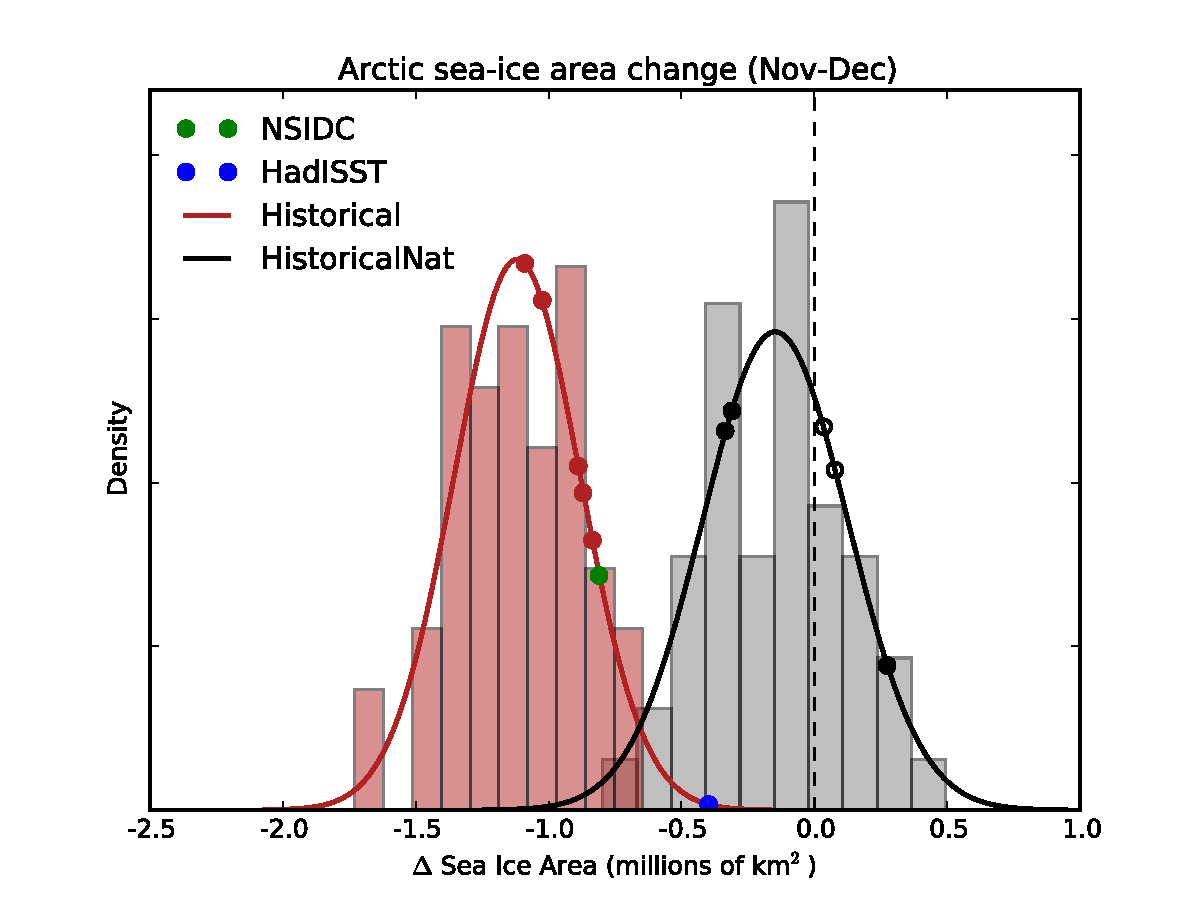
\includegraphics[width=20pc,angle=0]{fig1.pdf} \\ 
  \caption{CanESM large ensemble.
}\label{fig:fig1}
\end{figure}

\begin{figure}[t]
  \noindent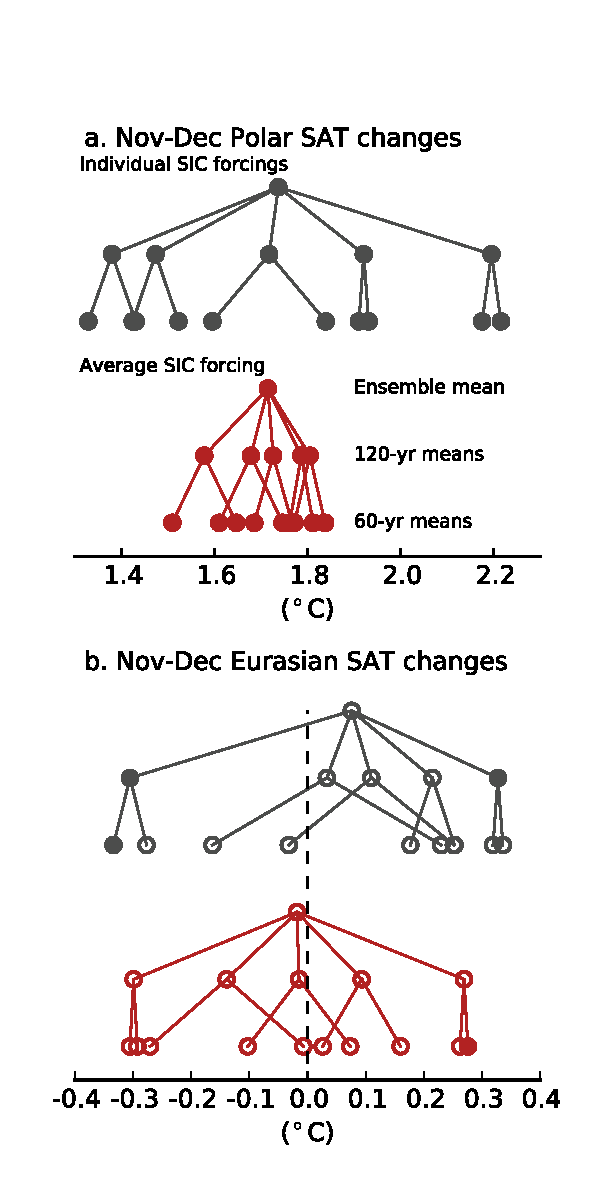
\includegraphics[width=19pc,angle=0]{fig2.pdf} \\ 
  \caption{Individual SIC forcings and Average SIC forcing uncertainty cascades.
}\label{fig:fig2}
\end{figure}

% Create a bibliography directory and place your .bib file there.
\clearpage
\bibliographystyle{./ametsoc}
\bibliography{./references}



\end{document}

